\documentclass[aspectratio=169,10pt]{beamer}
\usetheme{Madrid}
\usecolortheme{whale}

% --- Packages ---
\usepackage[utf8]{inputenc}
\usepackage[T1]{fontenc}
\usepackage{booktabs}
\usepackage{array}
\usepackage{amsmath,amssymb}
\usepackage{colortbl}
\usepackage{tikz}
\usetikzlibrary{automata, positioning, arrows.meta, shapes.geometric, calc}

% --- Custom Colors ---
\definecolor{gimpanavy}{RGB}{0, 43, 73}
\definecolor{gimpaaccent}{RGB}{30, 115, 190}
\definecolor{gimpalight}{RGB}{245, 247, 251}
\definecolor{gimpaheader}{RGB}{230, 238, 248}
\definecolor{darkred}{RGB}{180, 40, 40}
\definecolor{darkgreen}{RGB}{30, 140, 60}
\definecolor{papergold}{RGB}{210, 140, 10}

\setbeamercolor{palette primary}{bg=gimpanavy,fg=white}
\setbeamercolor{palette secondary}{bg=gimpaaccent,fg=white}
\setbeamercolor{palette tertiary}{bg=gimpanavy,fg=white}
\setbeamercolor{structure}{fg=gimpanavy}
\setbeamercolor{titlelike}{parent=structure,bg=gimpaheader}
\setbeamercolor{block title}{bg=gimpanavy,fg=white}
\setbeamercolor{block body}{bg=gimpalight}
\setbeamercolor{block title alerted}{bg=darkred,fg=white}
\setbeamercolor{block title example}{bg=darkgreen,fg=white}

% --- Title Information ---
\title[CS 305 $|$ Module 3]{Module 3: Computability, Undecidability \& System Limits}
\subtitle{CS 305: Theory of Computation (Weeks 9--12)}
\author[GIMPA School of Technology]{Department of Computer Science}
\institute[GIMPA]{Ghana Institute of Management and Public Administration (GIMPA)}
\date{Level 300 Undergraduate}

\begin{document}

% --- Title Slide ---
\begin{frame}
    \titlepage
\end{frame}

% --- Overview Slide ---
\begin{frame}{Module 3 Roadmap: Weeks 9 to 12}
    \begin{columns}[T]
        \column{0.48\textwidth}
        \begin{block}{Theoretical Foundations}
            \begin{itemize}\setlength{\itemsep}{3pt}
                \item \textbf{Wk 9:} Turing Machines (7-tuple) \& TM Variants
                \item \textbf{Wk 10:} The Church--Turing Thesis \& Algorithms
                \item \textbf{Wk 11:} Decidability of Regular/CFL Problems
                \item \textbf{Wk 12:} Halting Problem, Diagonalization \& Rice's Theorem
            \end{itemize}
        \end{block}
        
        \column{0.48\textwidth}
        \begin{alertblock}{Research Literature \& System Spotlights}
            \begin{itemize}\setlength{\itemsep}{3pt}
                \item \textbf{Wk 9:} \textbf{ICLR 2024 / ICML 2023:} Chain-of-Thought LLMs as Universal Turing Machines
                \item \textbf{Wk 10:} Universal Computation \& Physical Bounds
                \item \textbf{Wk 11:} \textbf{POPL / SLAM:} Static Code Verification
                \item \textbf{Wk 12:} \textbf{ACM CCS 2016:} Ethereum Gas Mechanics
            \end{itemize}
        \end{alertblock}
    \end{columns}
\end{frame}

% ==============================================================================
\section{Week 9: Turing Machines (TMs)}
% ==============================================================================

\begin{frame}{Week 9: Formal Definition of a Turing Machine}
    \begin{block}{Formal 7-Tuple Definition (Sipser Def 3.3)}
        A \textbf{Turing Machine (TM)} is a 7-tuple $(Q, \Sigma, \Gamma, \delta, q_0, q_{\text{accept}}, q_{\text{reject}})$:
        \begin{enumerate}
            \item $Q$ is the finite set of states.
            \item $\Sigma$ is the input alphabet (not containing blank symbol $\textvisiblespace$).
            \item $\Gamma$ is the tape alphabet ($\Sigma \subset \Gamma$ and $\textvisiblespace \in \Gamma$).
            \item $\delta: Q \times \Gamma \to Q \times \Gamma \times \{\text{L}, \text{R}\}$ is the transition function.
            \item $q_0 \in Q$ is the start state.
            \item $q_{\text{accept}} \in Q$ is the accept state.
            \item $q_{\text{reject}} \in Q$ is the reject state ($q_{\text{accept}} \neq q_{\text{reject}}$).
        \end{enumerate}
    \end{block}
    
    \begin{center}
    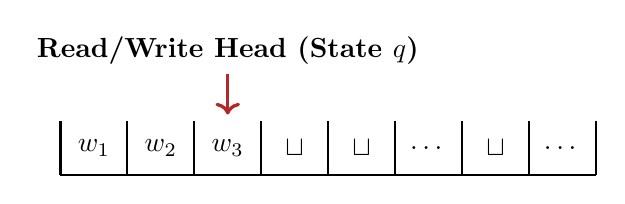
\begin{tikzpicture}[scale=0.85]
        \draw[thick] (0,0) grid (8,0.8);
        \node at (0.5,0.4) {$w_1$}; \node at (1.5,0.4) {$w_2$}; \node at (2.5,0.4) {$w_3$};
        \node at (3.5,0.4) {$\sqcup$}; \node at (4.5,0.4) {$\sqcup$};
        \node at (5.5,0.4) {$\dots$}; \node at (6.5,0.4) {$\sqcup$}; \node at (7.5,0.4) {$\dots$};
        \draw[->, very thick, color=darkred] (2.5, 1.5) -- (2.5, 0.9);
        \node[above] at (2.5, 1.5) {\textbf{Read/Write Head (State $q$)}};
    \end{tikzpicture}
    \end{center}
\end{frame}

\begin{frame}{Week 9 Research Spotlight: ICLR 2024 \& Turing Completeness of CoT}
    \begin{exampleblock}{Seminal Reading: ICLR 2024 / ICML 2023}
        \textbf{Merrill \& Sabharwal (Allen AI / Univ. of Washington)}, \textit{``The Expressive Power of Transformers with Chain of Thought,''} \textbf{ICLR 2024}; \textbf{Schuurmans et al. (Google Brain)}, \textbf{ICML 2023}.
    \end{exampleblock}
    
    \begin{columns}[T]
        \column{0.48\textwidth}
        \begin{block}{Transformer Without CoT (Direct Output)}
            \begin{itemize}
                \item Forward pass has fixed circuit depth $L$.
                \item Cannot iterate or execute unbounded dynamic steps.
                \item Strictly bounded in circuit complexity ($\textsf{TC}^0$).
            \end{itemize}
        \end{block}
        
        \column{0.48\textwidth}
        \begin{alertblock}{Transformer + Chain-of-Thought (Scratchpad)}
            \begin{itemize}
                \item Output tokens serve as an \textbf{infinite Turing read/write tape}.
                \item The model stores state, updates memory, and loops.
                \item \textbf{Proved Turing-Complete (Universal Computation)!}
            \end{itemize}
        \end{alertblock}
    \end{columns}
\end{frame}

% ==============================================================================
\section{Week 10: The Church--Turing Thesis}
% ==============================================================================

\begin{frame}{Week 10: The Church--Turing Thesis \& Robustness}
    \begin{block}{Theorem: Equivalence of Turing Machine Variants}
        The following models all recognize the \textbf{exact same class of languages}:
        \begin{itemize}
            \item Single-tape Deterministic Turing Machines
            \item Multi-tape Turing Machines (reading $k$ tapes simultaneously)
            \item Nondeterministic Turing Machines (NTMs)
            \item Random-Access Memory (RAM) computers, C, Python, Java, Lambda Calculus
        \end{itemize}
    \end{block}
    
    \begin{alertblock}{The Church--Turing Thesis}
        $$\text{Intuitive notion of an algorithm} \equiv \text{Turing Machine algorithm}$$
        \textit{Any algorithmic calculation that can be physically executed in the universe can be computed by a Turing Machine.}
    \end{alertblock}
\end{frame}

% ==============================================================================
\section{Week 11: Decidability}
% ==============================================================================

\begin{frame}{Week 11: Decidable vs. Recognizable Languages}
    \begin{columns}[T]
        \column{0.48\textwidth}
        \begin{block}{Turing-Recognizable (Recursively Enumerable)}
            A machine $M$ recognizes $L$ if for any string $w \in L$, $M$ halts and accepts. If $w \notin L$, $M$ may reject or \textbf{loop forever}.
        \end{block}
        
        \column{0.48\textwidth}
        \begin{exampleblock}{Turing-Decidable (Recursive)}
            A machine $M$ \textbf{decides} $L$ if $M$ halts on \textbf{every} input string (guaranteed never to loop).
            $$M(w) = \begin{cases} \text{Accept} & \text{if } w \in L \\ \text{Reject} & \text{if } w \notin L \end{cases}$$
        \end{exampleblock}
    \end{columns}
    
    \begin{block}{Decidable Problems Concerning Formal Languages (Sipser Ch. 4.1)}
        \begin{itemize}
            \item $A_{\text{DFA}} = \{\langle B, w \rangle \mid B \text{ is a DFA that accepts } w\}$ is \textbf{decidable}.
            \item $E_{\text{DFA}} = \{\langle B \rangle \mid B \text{ is a DFA and } L(B) = \varnothing\}$ is \textbf{decidable} (BFS graph reachability).
            \item $EQ_{\text{DFA}} = \{\langle A, B \rangle \mid A, B \text{ are DFAs and } L(A) = L(B)\}$ is \textbf{decidable} (symmetric difference).
        \end{itemize}
    \end{block}
\end{frame}

% ==============================================================================
\section{Week 12: Undecidability, Halting Problem \& Smart Contracts}
% ==============================================================================

\begin{frame}{Week 12: The Halting Problem \& Cantor's Diagonalization}
    \begin{block}{Theorem (Alan Turing, 1936; Sipser Thm 4.11)}
        $$A_{\text{TM}} = \{\langle M, w \rangle \mid M \text{ is a TM and } M \text{ accepts } w\} \quad \text{is \textbf{UNDECIDABLE}!}$$
    \end{block}
    
    \begin{columns}[T]
        \column{0.48\textwidth}
        \begin{alertblock}{Proof by Diagonal Contradiction}
            \begin{enumerate}\small
                \item Assume decider $H(\langle M, w \rangle)$ exists.
                \item Build opposite machine $D(\langle M \rangle)$:
                $$D(\langle M \rangle) = \begin{cases} \text{Reject} & \text{if } H(\langle M, \langle M \rangle \rangle) = \text{Accept} \\ \text{Accept} & \text{if } H(\langle M, \langle M \rangle \rangle) = \text{Reject} \end{cases}$$
                \item Run $D(\langle D \rangle) \implies$ $D$ accepts iff $D$ rejects! \textbf{Contradiction!}
            \end{enumerate}
        \end{alertblock}
        
        \column{0.48\textwidth}
        \begin{exampleblock}{Rice's Theorem (Sipser Problem 5.28)}
            \textbf{Any non-trivial semantic property of a Turing Machine's language is undecidable.}
            \begin{itemize}\small
                \item Is $L(M)$ empty? \textbf{Undecidable!}
                \item Is $L(M)$ regular? \textbf{Undecidable!}
                \item Does $M$ contain a virus? \textbf{Undecidable!}
            \end{itemize}
        \end{exampleblock}
    \end{columns}
\end{frame}

\begin{frame}{Week 12 Research Spotlight: ACM CCS 2016 \& Ethereum Smart Contracts}
    \begin{exampleblock}{Seminal Reading: ACM CCS 2016}
        \textbf{Luu et al. (National Univ. of Singapore)}, \textit{``Making Smart Contracts Smarter,''} \textbf{ACM Conference on Computer and Communications Security (CCS 2016)}.
    \end{exampleblock}
    
    \begin{columns}[T]
        \column{0.48\textwidth}
        \begin{block}{Case Study 1: Ethereum Smart Contract Gas}
            \begin{itemize}
                \item The EVM is Turing-complete.
                \item Miners cannot statically check if a contract has an infinite loop ($A_{\text{TM}}$ undecidable).
                \item \textbf{Solution:} Charge \textbf{Gas} for every execution opcode. If a contract loops, it runs out of gas and halts!
            \end{itemize}
        \end{block}
        
        \column{0.48\textwidth}
        \begin{alertblock}{Case Study 2: Anti-Virus Software Limitations}
            \begin{itemize}
                \item Can an AV company build a software analyzer that 100\% correctly identifies all malware?
                \item \textbf{No!} By Rice's Theorem (Cohen 1987), determining whether arbitrary binary code contains malware is undecidable.
            \end{itemize}
        \end{alertblock}
    \end{columns}
\end{frame}

% --- Summary Slide ---
\begin{frame}{Module 3 Summary \& Looking Ahead to Complexity}
    \begin{block}{Key Takeaways}
        \begin{itemize}\setlength{\itemsep}{3pt}
            \item \textbf{Turing Machines} define the absolute boundary of what algorithms can solve.
            \item Some problems are fundamentally \textbf{undecidable} (Halting problem, Rice's theorem) --- no amount of AI or compute power can ever solve them!
        \end{itemize}
    \end{block}
    
    \begin{exampleblock}{Looking Ahead: Module 4 (Computational Complexity \& Class NP)}
        For problems that \textit{are} decidable, can we solve them \textbf{efficiently in polynomial time}? $\to$ \textbf{$\mathbf{P}$ vs. $\mathbf{NP}$ and the Millenium Prize!}
    \end{exampleblock}
\end{frame}

\end{document}
